% Firestore collections and the Storage folder, with their links.
% Build: tectonic --outdir . fig-data-model-v1.tex
\documentclass[border=16pt]{standalone}
\usepackage[T1]{fontenc}
\usepackage[utf8]{inputenc}
\usepackage{helvet}
\renewcommand{\familydefault}{\sfdefault}
\usepackage[none]{hyphenat}
\usepackage{tikz}
\usetikzlibrary{arrows.meta,calc,shapes.geometric,shapes.multipart}

\definecolor{ink}{HTML}{0F2A33}
\definecolor{muted}{HTML}{5E7078}
\definecolor{line}{HTML}{C3CED2}
\definecolor{blue}{HTML}{1F5FA8}
\definecolor{hubfill}{HTML}{EDF2F4}

% A field line: name in typewriter, type in muted.
\newcommand{\fld}[2]{\texttt{#1}\hfill{\color{muted}#2}\\}
% A vector field, in blue.
\newcommand{\vfld}[2]{{\color{blue}\texttt{\textbf{#1}}}\hfill{\color{blue}#2}\\}

\begin{document}
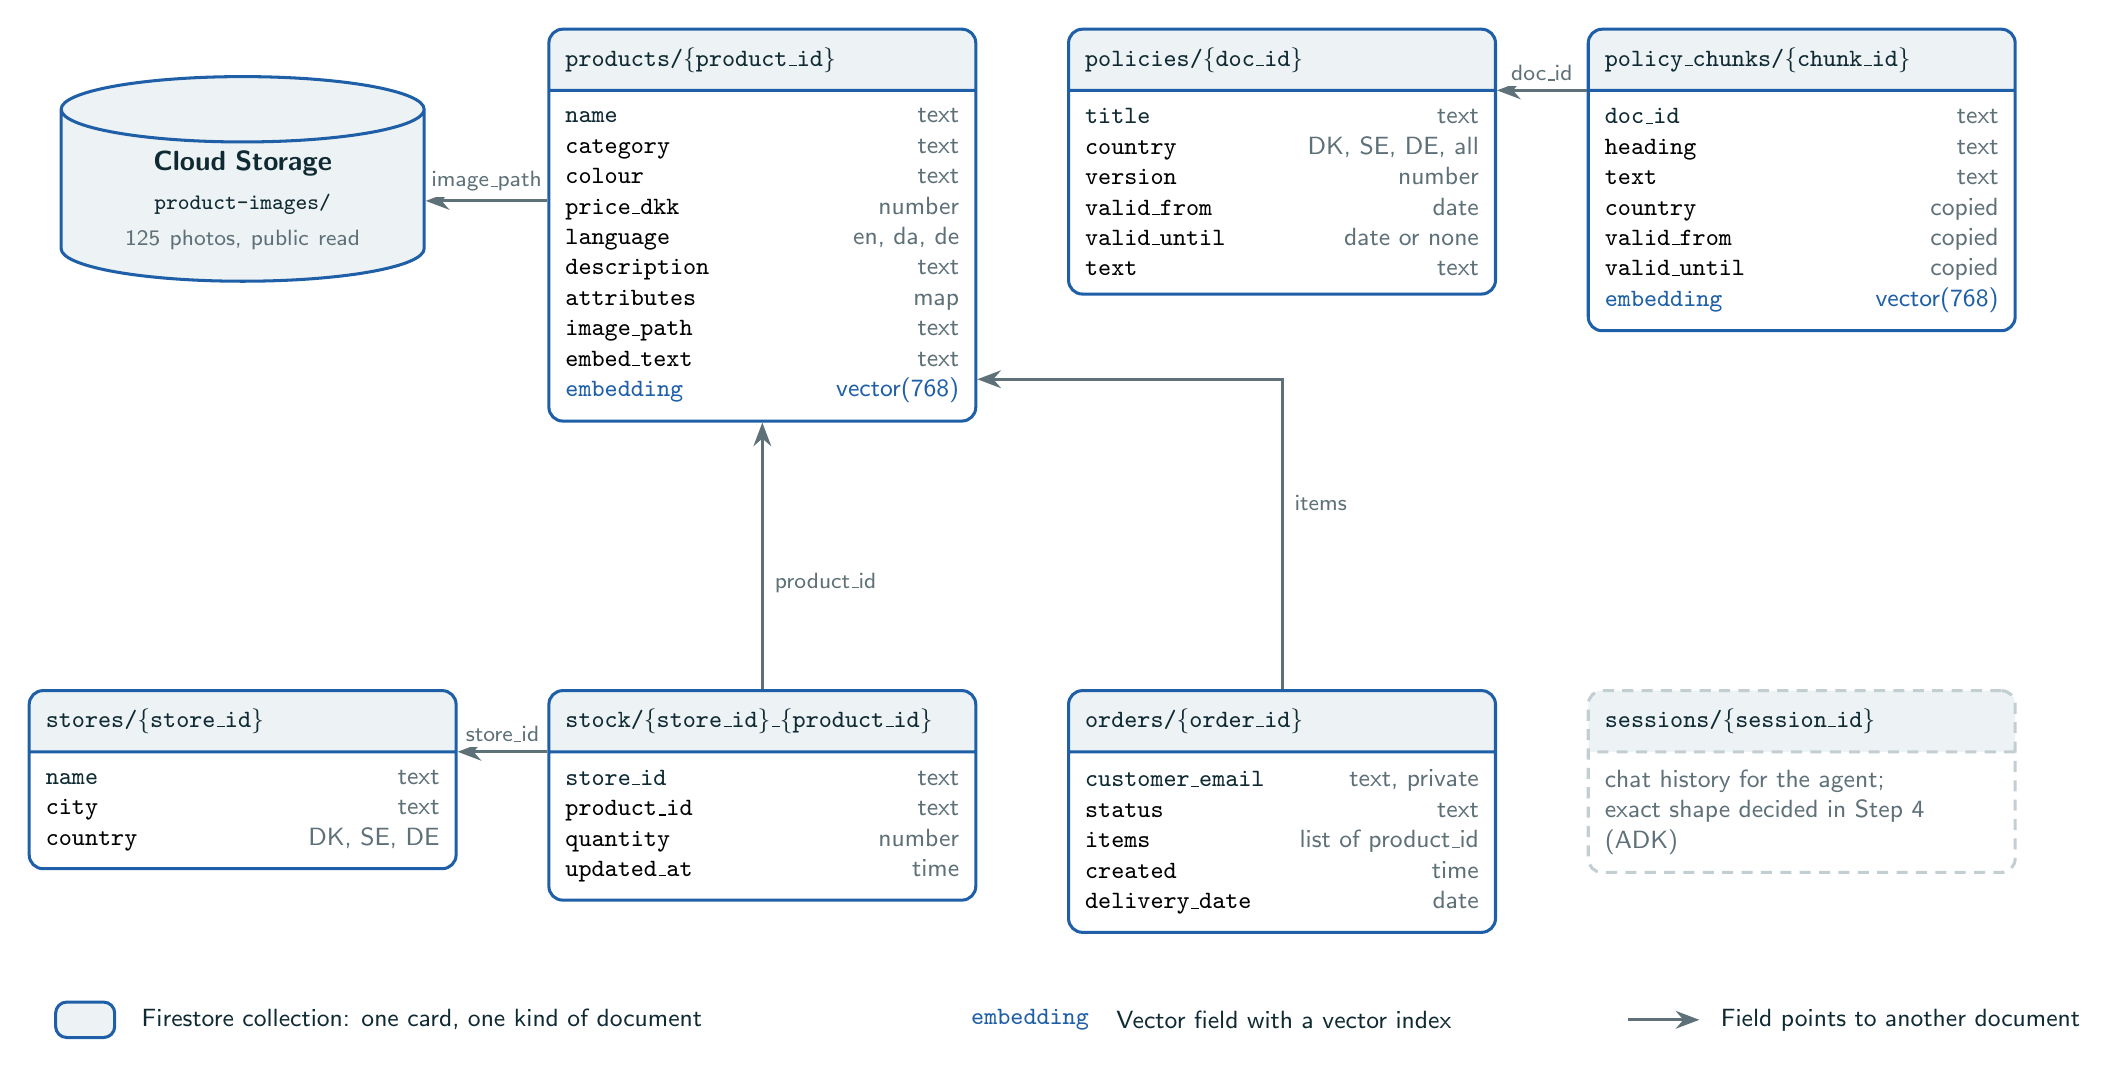
\begin{tikzpicture}[
  font=\sffamily,
  card/.style={rectangle split, rectangle split parts=2,
    rectangle split part fill={hubfill,white},
    rounded corners=5pt, draw=blue, line width=1.1pt, text=ink,
    text width=5.0cm, align=left, inner sep=6pt, font=\small\sffamily,
    anchor=north},
  ref/.style={line width=1.1pt, draw=muted, -{Stealth[length=3mm]}},
  store/.style={cylinder, shape border rotate=90, aspect=0.18,
    draw=blue, fill=hubfill, line width=1.1pt, text=ink, align=center,
    text width=4.4cm, minimum height=2.2cm, inner sep=3pt},
  note/.style={text=muted, font=\footnotesize\sffamily, fill=white,
    inner sep=2pt},
  zone/.style={text=muted, font=\large\sffamily},
]

% ---- Column positions ----
\def\ca{0}
\def\cb{6.6}
\def\cc{13.2}
\def\cd{19.8}

% ---- Top row ----
\node[card] (prod) at (\cb,0)
  {\textbf{\texttt{products/\{product\_id\}}}
   \nodepart{two}
   \fld{name}{text}
   \fld{category}{text}
   \fld{colour}{text}
   \fld{price\_dkk}{number}
   \fld{language}{en, da, de}
   \fld{description}{text}
   \fld{attributes}{map}
   \fld{image\_path}{text}
   \fld{embed\_text}{text}
   \vfld{embedding}{vector(768)}};

\node[card] (pol) at (\cc,0)
  {\textbf{\texttt{policies/\{doc\_id\}}}
   \nodepart{two}
   \fld{title}{text}
   \fld{country}{DK, SE, DE, all}
   \fld{version}{number}
   \fld{valid\_from}{date}
   \fld{valid\_until}{date or none}
   \fld{text}{text}};

\node[card] (chunk) at (\cd,0)
  {\textbf{\texttt{policy\_chunks/\{chunk\_id\}}}
   \nodepart{two}
   \fld{doc\_id}{text}
   \fld{heading}{text}
   \fld{text}{text}
   \fld{country}{copied}
   \fld{valid\_from}{copied}
   \fld{valid\_until}{copied}
   \vfld{embedding}{vector(768)}};

\node[store] (img) at (\ca,-2.2)
  {\textbf{Cloud Storage}\\[2pt]
   {\footnotesize\texttt{product-images/}}\\[1pt]
   {\footnotesize\color{muted}125 photos, public read}};

% ---- Bottom row ----
\def\yb{-8.4}
\node[card] (stores) at (\ca,\yb)
  {\textbf{\texttt{stores/\{store\_id\}}}
   \nodepart{two}
   \fld{name}{text}
   \fld{city}{text}
   \fld{country}{DK, SE, DE}};

\node[card] (stock) at (\cb,\yb)
  {\textbf{\texttt{stock/\{store\_id\}\_\{product\_id\}}}
   \nodepart{two}
   \fld{store\_id}{text}
   \fld{product\_id}{text}
   \fld{quantity}{number}
   \fld{updated\_at}{time}};

\node[card] (orders) at (\cc,\yb)
  {\textbf{\texttt{orders/\{order\_id\}}}
   \nodepart{two}
   \fld{customer\_email}{text, private}
   \fld{status}{text}
   \fld{items}{list of product\_id}
   \fld{created}{time}
   \fld{delivery\_date}{date}};

\node[card, draw=line, dashed, dash pattern=on 4pt off 3pt] (sess) at (\cd,\yb)
  {\textbf{\texttt{sessions/\{session\_id\}}}
   \nodepart{two}
   {\color{muted}chat history for the agent;\\
    exact shape decided in Step 4 (ADK)}};

% ---- Links: field refers to a document ----
\draw[ref] (prod.west |- img.east) -- node[note, above=1pt] {image\_path} (img.east);
\draw[ref] (chunk.text split west) -- node[note, above=1pt] {doc\_id}
  (chunk.text split west -| pol.east);
\draw[ref] (stock.north) -- node[note, right=2pt, pos=0.4] {product\_id}
  (stock.north |- prod.south);
\draw[ref] (stock.west |- stores.text split) -- node[note, above=1pt] {store\_id}
  (stores.east |- stores.text split);
\draw[ref] (orders.north) |- node[note, right=2pt, pos=0.3] {items}
  ([yshift=0.55cm]prod.south east);

% ---- Legend ----
\def\yl{-12.6}
\node[rounded corners=4pt, draw=blue, line width=1.1pt, fill=hubfill,
      minimum width=0.75cm, minimum height=0.45cm] (k1) at (\ca-2.0,\yl) {};
\node[anchor=west, text=ink, font=\small] at ([xshift=0.2cm]k1.east)
  {Firestore collection: one card, one kind of document};
\node[text=blue, font=\small\bfseries\ttfamily] (k2) at (\cb+3.4,\yl) {embedding};
\node[anchor=west, text=ink, font=\small] at ([xshift=0.1cm]k2.east)
  {Vector field with a vector index};
\draw[ref] (\cc+4.4,\yl) -- (\cc+5.3,\yl);
\node[anchor=west, text=ink, font=\small] at (\cc+5.45,\yl)
  {Field points to another document};

\end{tikzpicture}
\end{document}
